Существует огромное разнообразие методов балансировки. 
Рассмотренные в данной работе представленны в схеме (см. \figurename\ref{fig:classification}). \\

Все методы можно условно поделить на активную и пассивную. \\
\textbf{Пассивная балансировка ---}  это метод уравновешивает ячейки только во время заряда 
путем рассеивания избыточной энергии в виде тепла.
Этот метод дешевый и простой. \\
\textbf{Активная балансировка ---} предполагает активное перераспределение энергии между ячейками. 
Энергия не уходит в тепло, как в пассивном методе.
Работает всё время. 

Еще сушествует так называемая \textbf{балансировка \glqq без потерь\grqq}, говоря по простому блоки батареи поочередно разряжаются,
тем самым вся энергия ячеек расходуется без потерь, при зарядке аналогичная процедура. Этот метод будет расмотрен отдельно от других.

\begin{figure}[h]
    \centering
    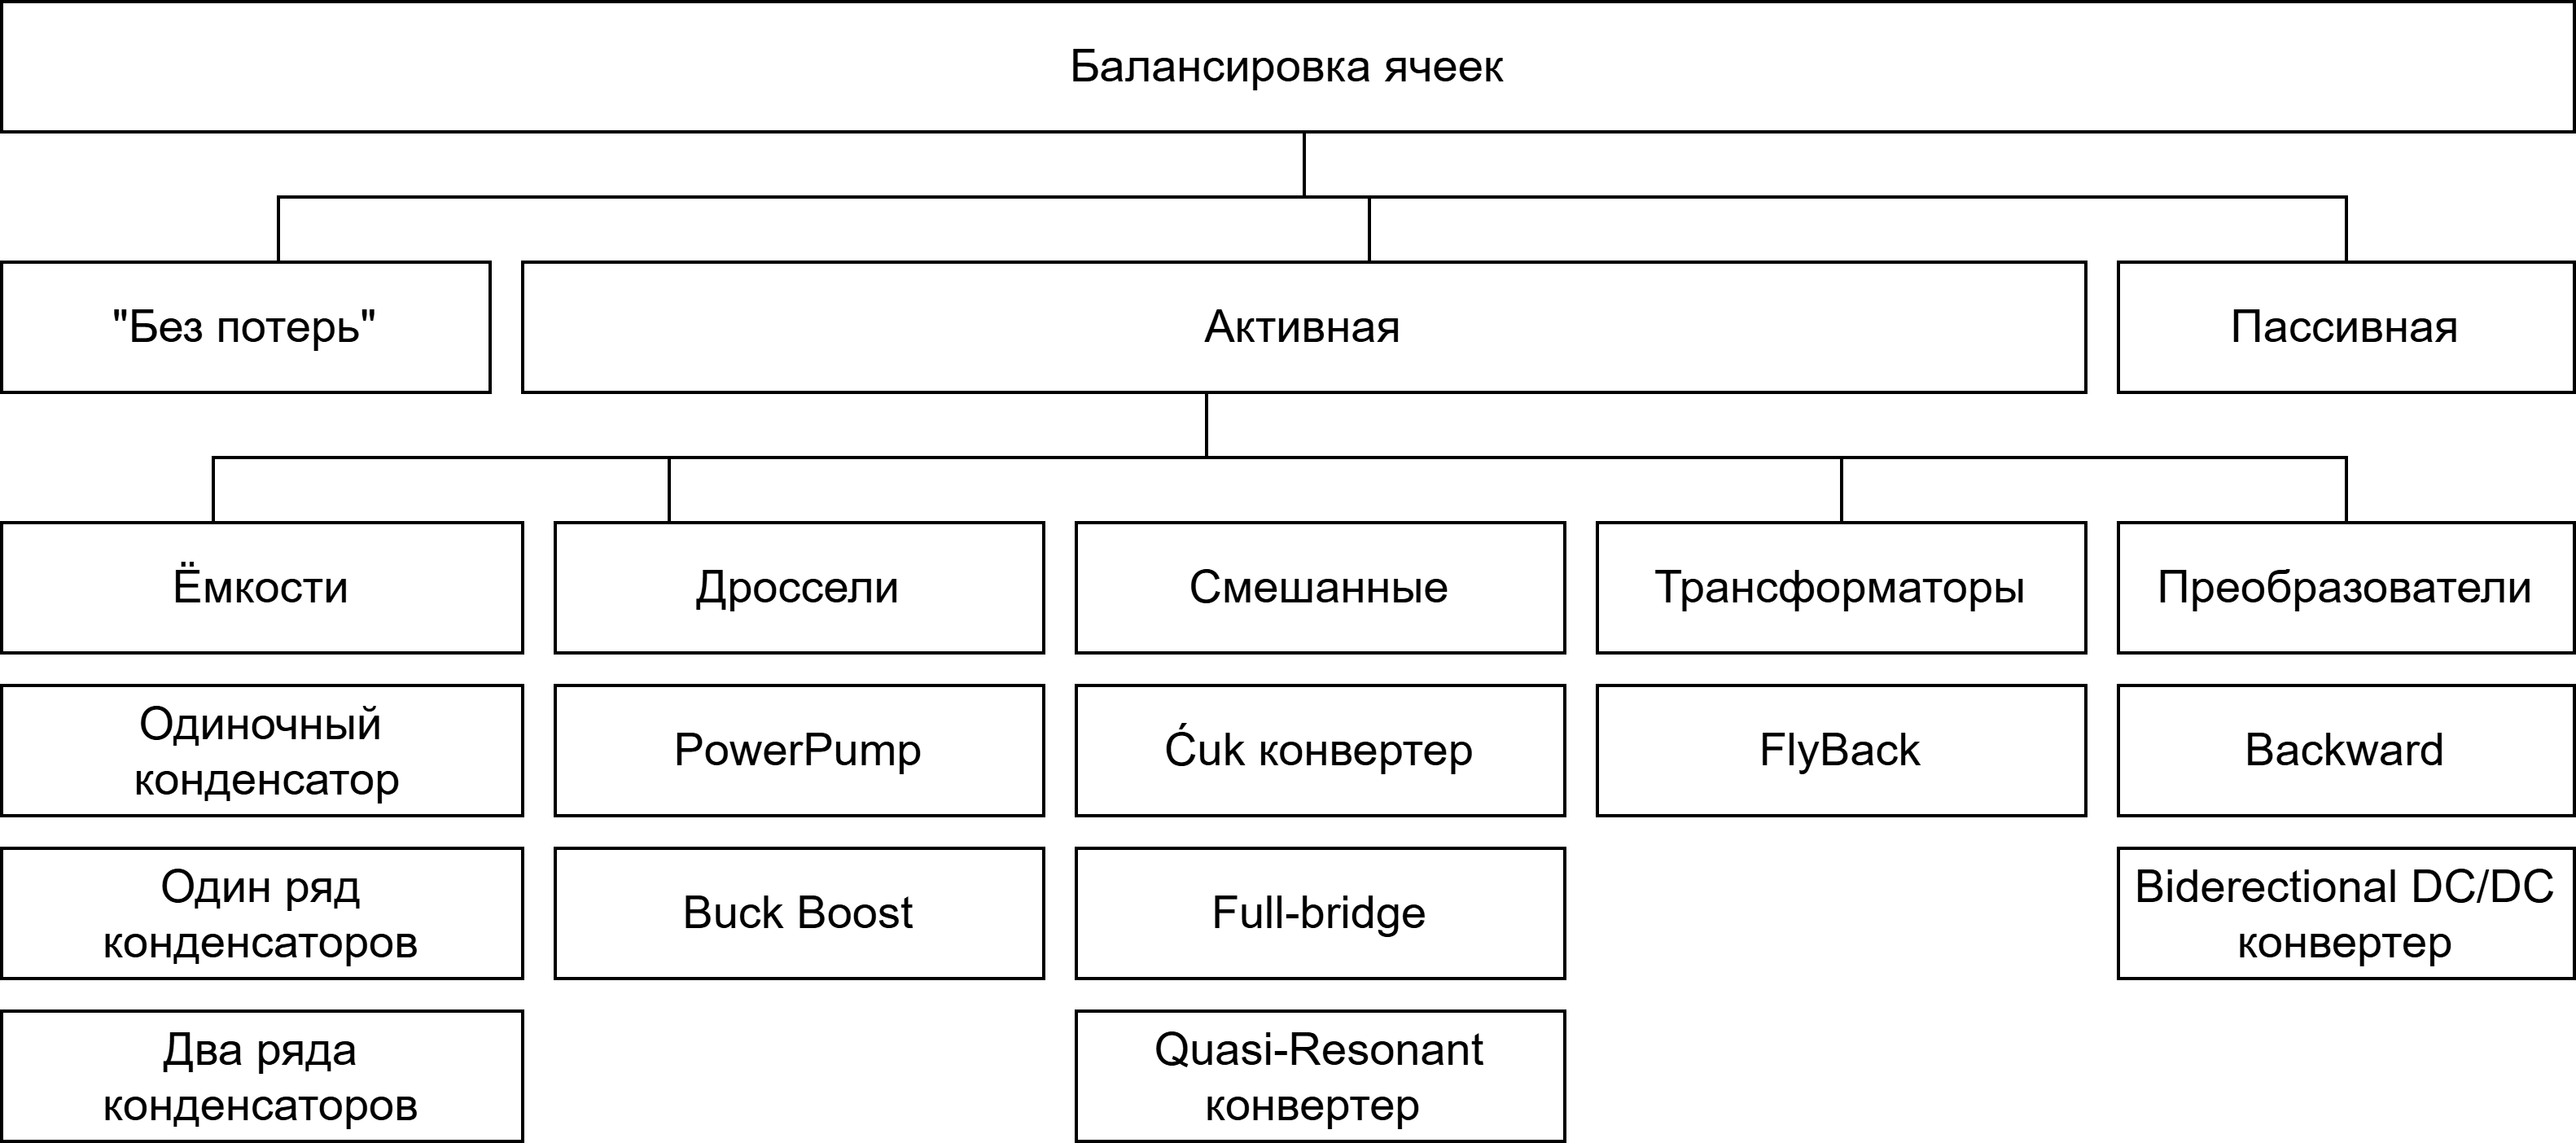
\includegraphics[width=\linewidth]{img/classification.png}
    \caption{Схема сущевствующих методов балансировки}
    \label{fig:classification}
\end{figure}


\subsection{Пассивная балансировка}
\input{notes/rewiew/passive_balacing.tex}

\subsection{Активная балансировка}
В методах активной балансировки используются различные накопители энергии.
Которые служат временным буффером для энергии.
Алгоритм зарядки перенаправляет энергию от перезаряженной ячейке к менее заряженной.
Основные элементы таких схем это конденсаторы, дроссели, трансформаторы. 
Так же используются dc/dc преобразователи.

\subsection{Балансировка \glqq без потерь\grqq}
Идея данного метода балансировки достаточно проста.
Батарея состоит из нескольких последовательных блоков и ключей.
Ключи установленны таким образом, чтобы включать/выключать конкретную ячейку из общей сети.

\begin{figure}[!h]
    \centering
    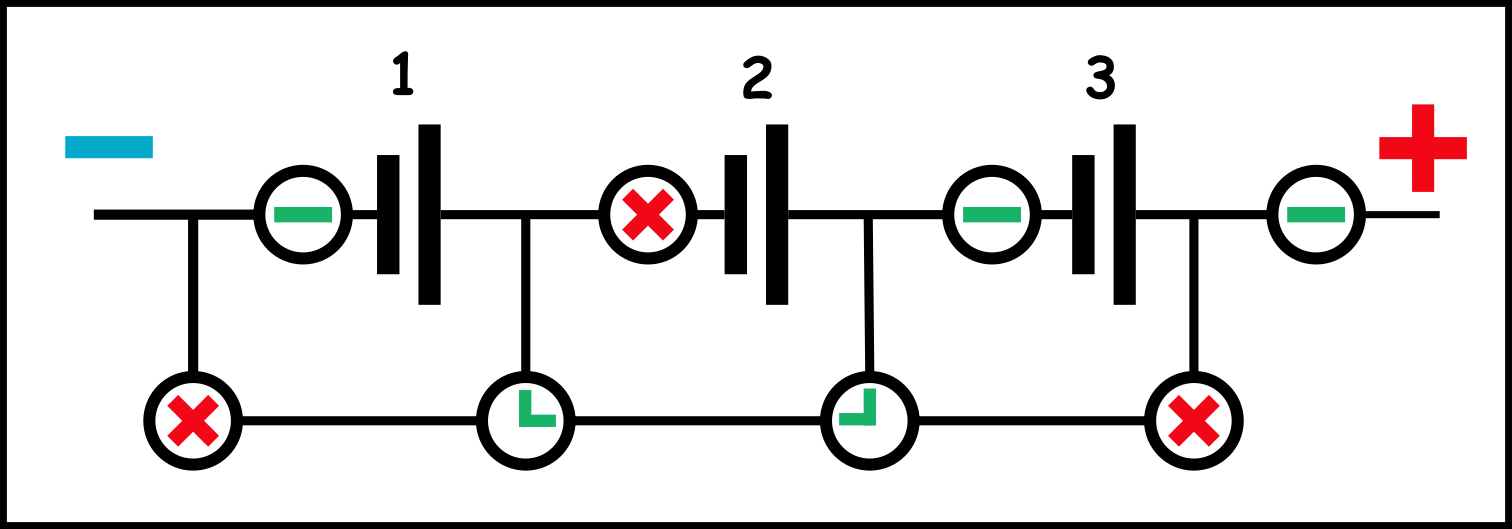
\includegraphics[width=0.7\linewidth]{img/no_loss_balancing.png}
    \caption{Принципиальная схема для балансировки "без потерь"}
    \label{fig:no_loss}
\end{figure}
